\documentclass[pnumromarab,times]{politex}

% ========== Packages ==========
\usepackage[utf8]{inputenc}
\usepackage{amsmath,amsthm,amsfonts,amssymb}
\usepackage{graphicx,enumerate}
\graphicspath{{imgs/}}
\usepackage[brazil]{babel}
\usepackage{url}
\usepackage{booktabs}
\usepackage{tikz}
\usetikzlibrary{positioning,arrows.meta,calc}
\usepackage[num]{abntex2cite}   % referências no padrão ABNT (NBR 6023), sistema numérico

% ========== Opções do documento ==========
\titulo{Reprodução da Arquitetura do Game Boy Advance em FPGA}

\autor{Caio Jun Takahashi, 12488380}

\orientador{Prof.\ Dr.\ Bruno Cavalcante de Souza Sanches}

% Trabalho de Conclusão de Curso da Escola Politécnica da USP.
% [INDICAR: confirmar a ênfase exata do curso junto à coordenação;
%  o valor abaixo segue o padrão do departamento PSI/PCS.]
\tcc{Engenharia Elétrica com ênfase em Sistemas Eletrônicos}

\departamento{Departamento de Engenharia de Sistemas Eletrônicos (PSI)}
\areaConcentracao{Sistemas Eletrônicos}

\local{São Paulo}
\data{2026}


\begin{document}
% ========== Capa e folhas de rosto ==========
\capa
\falsafolhaderosto
\folhaderosto


% ========== Dedicatória (opcional) ==========
% [OPCIONAL: incluir dedicatória pessoal antes da entrega final.]
% \dedicatoria{Dedicatória}


% ========== Agradecimentos ==========
%\begin{agradecimentos}
%% [INDICAR: redigir agradecimentos pessoais ao orientador, familiares
%%  e demais colaboradores antes da entrega final.]
%Ao orientador, Prof.\ Dr.\ Bruno Cavalcante de Souza Sanches, pela
%disponibilidade, paciência e direcionamento técnico ao longo do
%desenvolvimento deste trabalho. Aos professores da Escola Politécnica
%que contribuíram, ao longo da graduação, com a base teórica em
%sistemas digitais, arquitetura de computadores e projeto de hardware
%indispensável à realização do projeto. Aos colegas e familiares pelo
%apoio durante a execução do Trabalho de Conclusão de Curso.
%\end{agradecimentos}


% ========== Epígrafe (opcional) ==========


% ========== Resumo ==========
\begin{resumo}
Este trabalho propõe a reprodução da arquitetura do console portátil
Game Boy Advance (GBA) em uma plataforma de hardware reconfigurável
do tipo FPGA. O objetivo é descrever em \emph{Verilog} os principais
blocos funcionais do console, o núcleo de processamento ARM7TDMI,
o subsistema de memória (BIOS, EWRAM, IWRAM, VRAM, OAM e Palette RAM),
o controlador de barramento e, em etapa posterior, a unidade de
processamento gráfico e a interface de saída de vídeo, de modo que
o sistema integrado seja capaz de executar programas binários
originalmente compilados para o GBA. A implementação é validada na
placa Altera DE1-SoC, que contém uma FPGA Cyclone V, utilizando o
fluxo de projeto Quartus Prime, simulação no ModelSim/QuestaSim e
\textit{toolchain} \texttt{arm-none-eabi} para a geração de programas
de teste em \emph{assembly} ARM e Thumb. Diferentemente da emulação
puramente em software, a abordagem proposta procura preservar a
temporização e o comportamento original do hardware, o que confere
maior fidelidade à reprodução e, ao mesmo tempo, permite um estudo
aprofundado de arquitetura de computadores e de projeto de sistemas
digitais. No estágio atual do desenvolvimento, correspondente à
presente entrega intermediária, o núcleo ARM7TDMI já se encontra
implementado e validado, tanto em simulação quanto em hardware, e
constitui a prova de conceito apresentada neste momento. O subsistema
de memória, mapa de memória do GBA, controlador e árbitro de
barramento, canais de DMA e controlador de SDRAM para a ROM de
cartucho e a EWRAM, já se encontra descrito e integrado ao \textit{datapath},
com a validação funcional do caminho integrado ainda em andamento; o
subsistema de vídeo e a integração final permanecem como continuidade
prevista do trabalho.
%
\\[3\baselineskip]
%
\textbf{Palavras-Chave}, FPGA, Game Boy Advance, ARM7TDMI,
Arquitetura de Computadores, Verilog, Sistemas Digitais Reconfiguráveis.
\end{resumo}


% ========== Abstract ==========
\begin{abstract}
This work proposes the reproduction of the Game Boy Advance (GBA)
portable console architecture on a reconfigurable FPGA platform. The
goal is to describe in \emph{Verilog} the main functional blocks of
the console, the ARM7TDMI processing core, the memory subsystem
(BIOS, EWRAM, IWRAM, VRAM, OAM and Palette RAM), the bus controller
and, in a later stage, the graphics processing unit and the video
output interface, so that the integrated system is able to execute
binary programs originally compiled for the GBA. The implementation
is validated on the Altera DE1-SoC board, which carries a Cyclone V
FPGA, using the Quartus Prime design flow, ModelSim/QuestaSim
simulation and the \texttt{arm-none-eabi} toolchain to produce ARM
and Thumb assembly test programs. Differently from purely software
emulation, the proposed approach aims to preserve the original
timing and behaviour of the hardware, which provides a higher
fidelity reproduction and, at the same time, allows a deeper study
of computer architecture and digital system design. At the current
development stage, corresponding to this intermediate delivery, the
ARM7TDMI core is already implemented and validated, both in
simulation and on hardware, and constitutes the proof of concept
presented at this point. The memory subsystem, the GBA memory map,
the bus controller and arbiter, the DMA channels and an SDRAM controller
for the cartridge ROM and EWRAM, is already described and integrated into the
datapath, with functional validation of the integrated path still
ongoing; the video subsystem and the final integration remain the
planned continuation of the work.
%
\\[3\baselineskip]
%
\textbf{Keywords}, FPGA, Game Boy Advance, ARM7TDMI, Computer
Architecture, Verilog, Reconfigurable Digital Systems.
\end{abstract}


% ========== Listas (opcional) ==========
% [INDICAR: \listadefiguras só faz sentido após a inserção das
%  figuras (diagrama de blocos do sistema, fluxo do datapath,
%  diagrama de tempo, etc.). Manter comentado até inclusão.]
\listadefiguras
%\listadetabelas


% ========== Lista de símbolos e siglas ==========
\begin{pretextualsection}{Lista de Siglas}
\begin{description}
    \item[ALU] Arithmetic Logic Unit
    \item[ARM] Advanced RISC Machines
    \item[ASIC] Application-Specific Integrated Circuit
    \item[BIOS] Basic Input/Output System
    \item[CPSR] Current Program Status Register
    \item[CPU] Central Processing Unit
    \item[DMA] Direct Memory Access
    \item[EWRAM] External Work RAM
    \item[FPGA] Field-Programmable Gate Array
    \item[GBA] Game Boy Advance
    \item[GPU] Graphics Processing Unit
    \item[HDL] Hardware Description Language
    \item[IRQ] Interrupt Request
    \item[IWRAM] Internal Work RAM
    \item[OAM] Object Attribute Memory
    \item[PC] Program Counter
    \item[PLL] Phase-Locked Loop
    \item[PPU] Picture Processing Unit
    \item[RAM] Random Access Memory
    \item[ROM] Read-Only Memory
    \item[RTL] Register Transfer Level
    \item[SoC] System-on-Chip
    \item[SPSR] Saved Program Status Register
    \item[SRAM] Static Random Access Memory
    \item[SDRAM] Synchronous Dynamic Random Access Memory
    \item[VGA] Video Graphics Array
    \item[VRAM] Video RAM
\end{description}
\end{pretextualsection}


% ========== Sumário ==========
\sumario



% ========== Elementos textuais ==========

\chapter{Introdução}
\label{cap:introducao}

\section{Antecedentes}
\label{sec:antecedentes}

O Game Boy Advance (GBA), lançado pela Nintendo em 2001, foi o sucessor
direto do Game Boy Color e representou um salto arquitetural relevante
na linha de consoles portáteis da empresa. Diferentemente de seus
predecessores, baseados em variações do Z80, o GBA adota como núcleo
principal o processador ARM7TDMI, um \emph{core} RISC de 32~bits
desenvolvido pela ARM Limited e largamente utilizado em sistemas
embarcados da primeira metade da década de 2000~\cite{ARM_DDI0210B,
ARM_DVI0027B}. Em complemento, o console preserva um co-processador
Sharp~LR35902 (compatível com o Game Boy Color) para retrocompatibilidade
com a biblioteca anterior, bem como blocos dedicados a vídeo, áudio e
acesso direto à memória~\cite{Copetti2019,Vijn_Tonc}. A
Figura~\ref{fig:gba-console} apresenta o aparelho em sua forma original.

\begin{figure}[htbp]
    \centering
    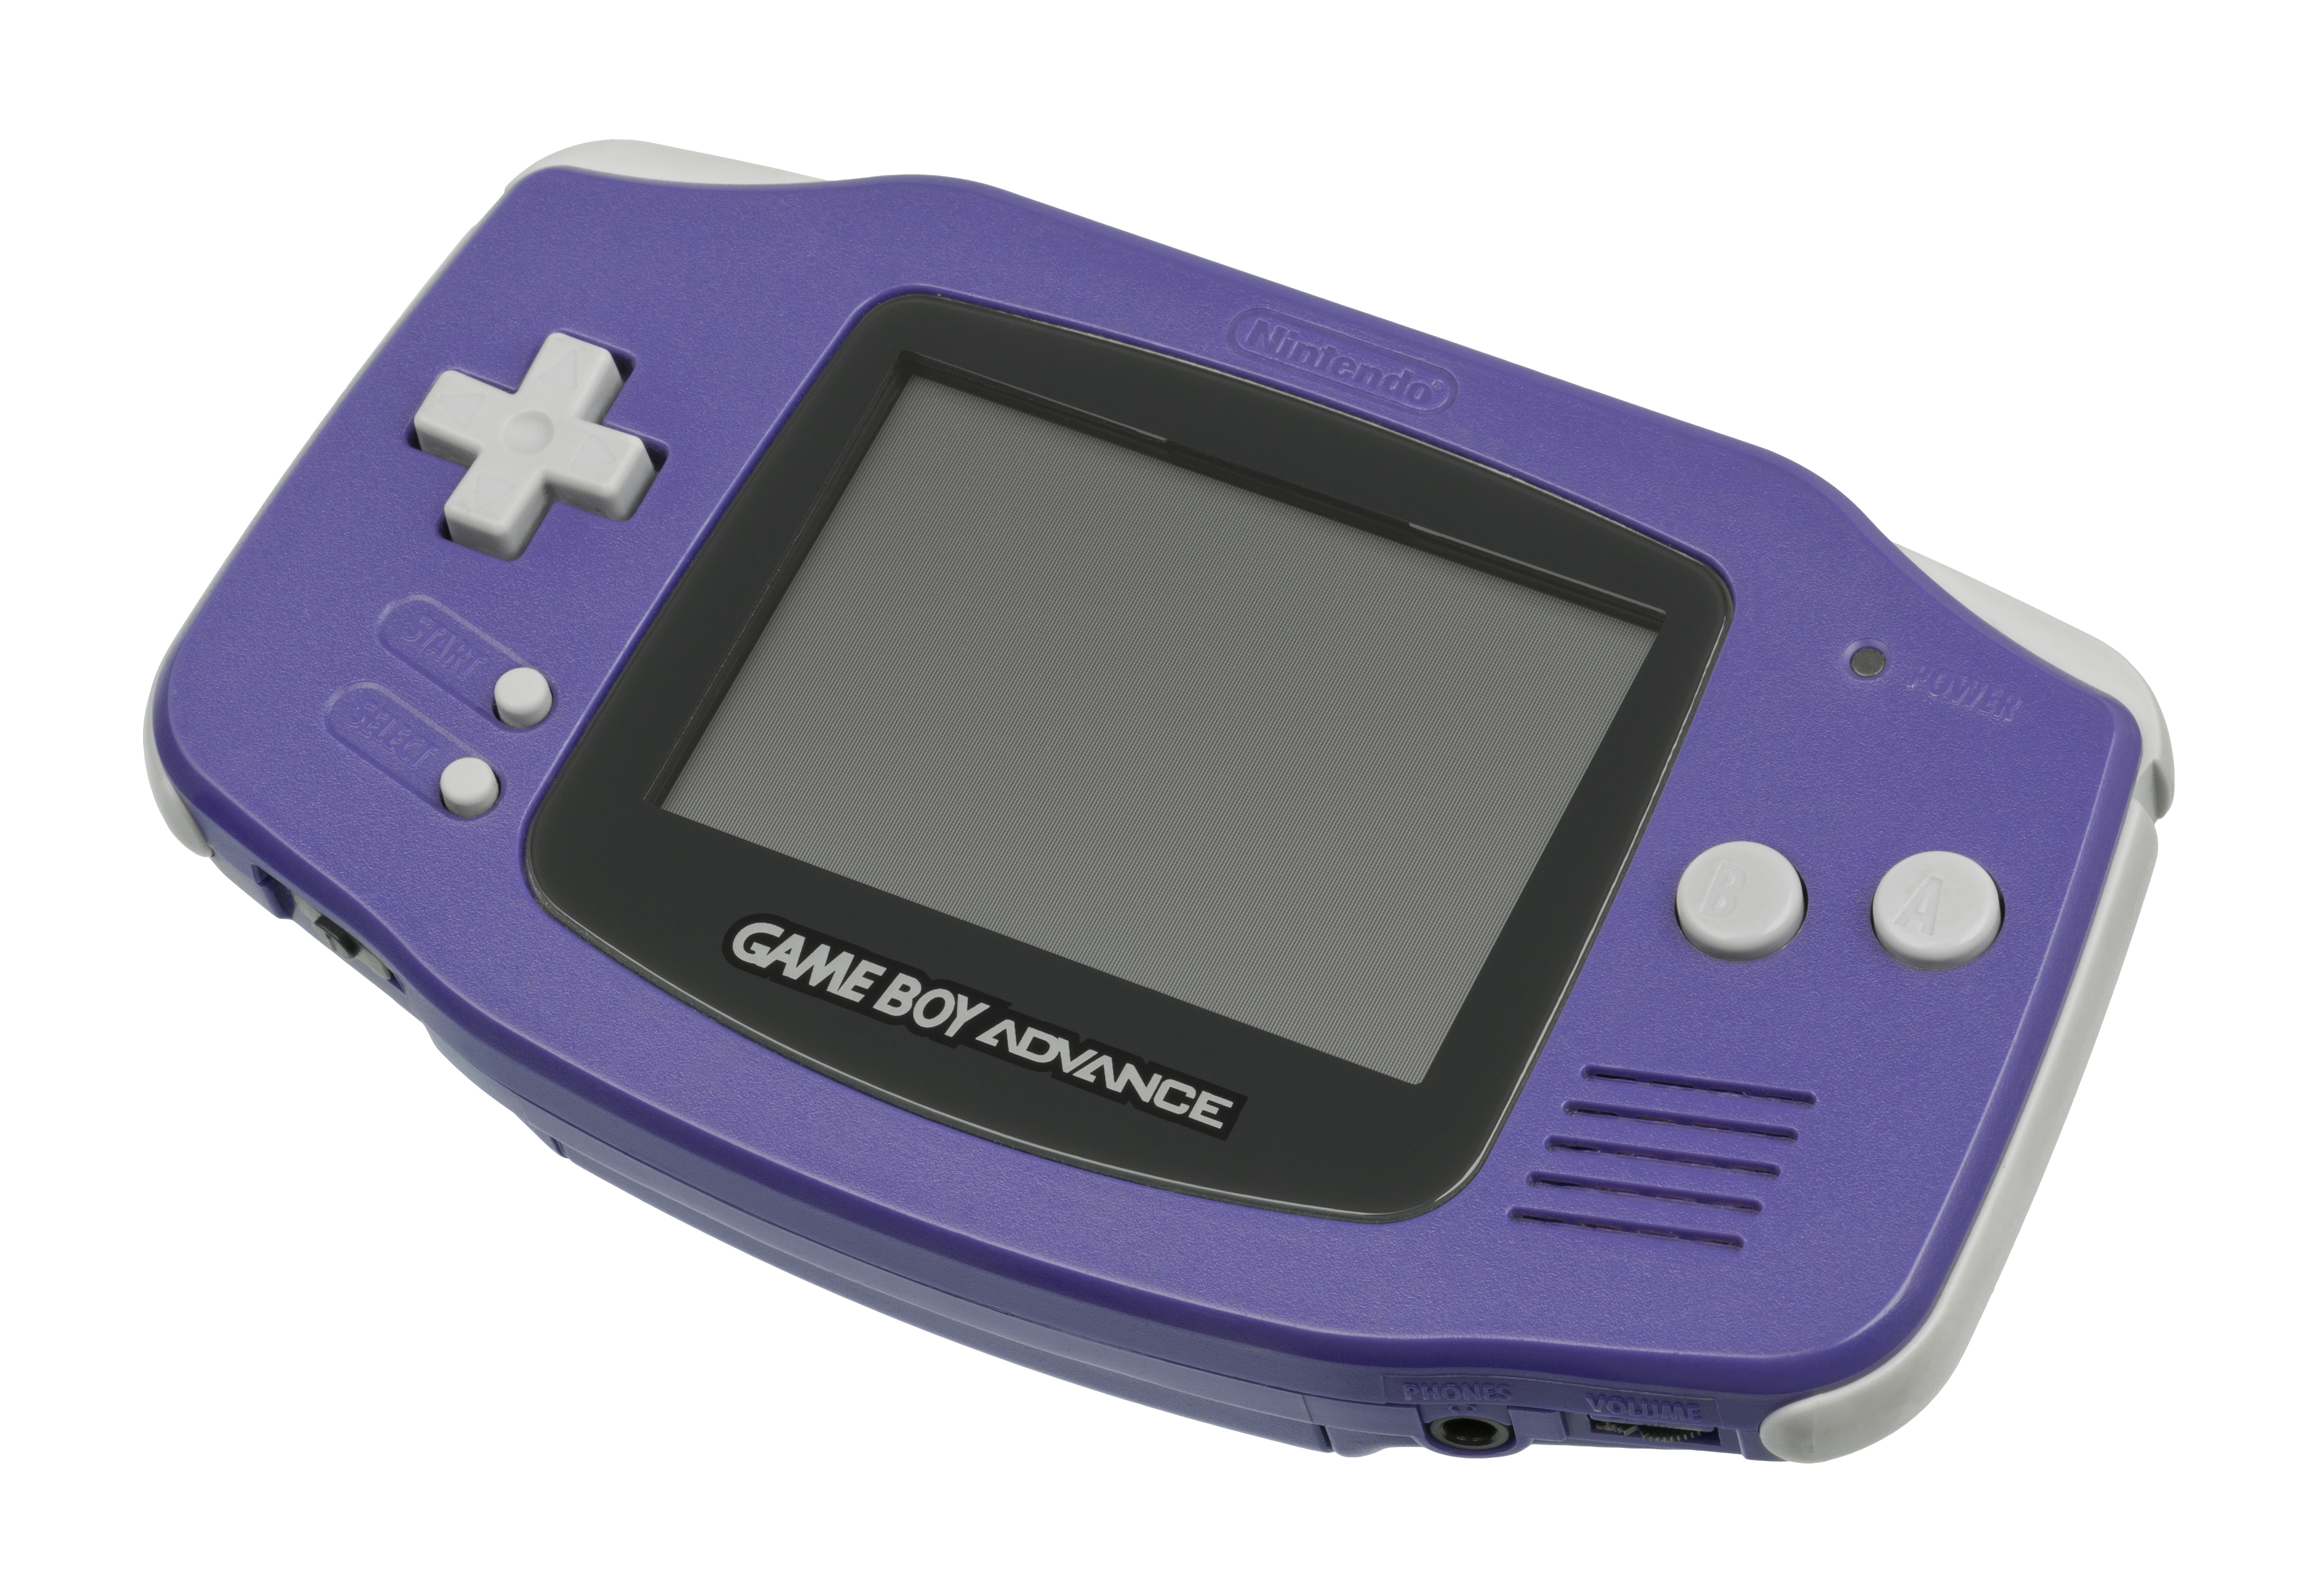
\includegraphics[width=0.55\textwidth]{Nintendo-Game-Boy-Advance-Purple-FL.jpg}
    \caption{Console Game Boy Advance (modelo AGB-001), lançado pela Nintendo
        em 2001.
        Fonte: Wikimedia Commons (domínio público).}
    \label{fig:gba-console}
\end{figure}

A arquitetura do GBA combina, portanto, um processador de uso geral,
um espaço de endereçamento segmentado em múltiplas regiões com
características distintas de largura, latência e função (BIOS, EWRAM,
IWRAM, registradores de I/O, Palette RAM, VRAM, OAM, ROM de cartucho
e SRAM de salvamento) e uma PPU capaz de operar em seis modos
gráficos distintos, alguns baseados em \emph{tilemaps} e outros em
\emph{bitmaps}~\cite{Copetti2019,Vijn_Tonc,GBATEK}. Esse conjunto
torna o console uma plataforma compacta, porém arquiteturalmente
rica, e didaticamente interessante para o estudo de organização de
computadores e projeto de sistemas digitais.

Do ponto de vista tecnológico, as últimas duas décadas viram o
amadurecimento das FPGAs como veículo de reprodução fiel de
arquiteturas históricas. Diferentemente da emulação por software,
em que o comportamento do hardware original é \emph{imitado} por
um programa executado sobre um processador moderno, a implementação
em FPGA descreve, em linguagem de descrição de hardware (HDL), os
blocos digitais que compõem o sistema, sintetizando-os em uma malha
de células lógicas reconfiguráveis~\cite{PattersonHennessy,
HarrisHarris}. O resultado é um sistema digital efetivamente
equivalente ao original do ponto de vista da temporização e do
comportamento ciclo a ciclo, ainda que materializado em um
\textit{die} distinto.


\section{Motivação}
\label{sec:motivacao}

A motivação para o desenvolvimento deste trabalho parte de três
vetores convergentes. O primeiro é a \textbf{preservação histórica}:
o GBA é um console descontinuado desde 2010, cujo \textit{die}
original (\textit{Custom CPU Agb}) não é mais fabricado e cujos
exemplares em bom estado de conservação se tornam progressivamente
escassos e caros no mercado de usados~\cite{Copetti2019}. O segundo
vetor é \textbf{didático}: a reprodução em hardware reconfigurável
da arquitetura do console exige a aplicação integrada de conhecimentos
de arquitetura de computadores, projeto digital, verificação funcional,
ferramentas de EDA e \textit{toolchains} de \textit{cross-compilation},
o que o torna um projeto de Conclusão de Curso de elevado retorno
formativo. O terceiro vetor é \textbf{tecnológico}: trabalhos como
MiSTer FPGA~\cite{MiSTer} e Analogue Pocket~\cite{AnaloguePocket}
demonstraram que FPGAs de custo acessível são hoje capazes de
hospedar reproduções completas de consoles da era 8/16/32~bits,
configurando uma fronteira ativa e viável de pesquisa aplicada.


\section{Relevância}
\label{sec:relevancia}

A relevância deste trabalho manifesta-se em três frentes
complementares. Do ponto de vista \textbf{acadêmico}, o projeto
percorre, de ponta a ponta, o ciclo de vida de um sistema digital
não trivial: parte da especificação extraída da documentação técnica
original do processador~\cite{ARM_DDI0210B,ARM_DVI0027B} e do
console~\cite{GBATEK,Copetti2019}, passa pela descrição RTL em
\emph{Verilog} e culmina na verificação por simulação e na síntese
física em FPGA real. Do ponto de vista \textbf{preservacionista}, e
ao contrário de uma emulação em software, a implementação em FPGA
preserva diretamente o \emph{comportamento} do hardware original,
sua estrutura de barramento, sua hierarquia de memória e suas
relações de temporização~\cite{HarrisHarris}, contribuindo para
a documentação viva de uma arquitetura que tende a se perder com o
tempo. Por fim, do ponto de vista \textbf{tecnológico}, o
desenvolvimento abre caminho para extensões futuras, como a
inclusão de interface de cartucho físico, áudio e controle externo,
ou a portabilidade para FPGAs de menor custo, demonstrando que
projetos de nicho podem ser realizados com os recursos didáticos
disponíveis em ambiente universitário.


\section{Declaração do Problema}
\label{sec:problema}

A execução fiel de jogos originalmente publicados para o GBA
depende, hoje, ou (i) da disponibilidade do console físico original,
cuja oferta no mercado é decrescente e cujo custo é crescente; ou
(ii) de emuladores em software que, embora maduros, executam-se
sobre processadores de propósito geral e introduzem desvios de
temporização e comportamento difíceis de auditar
\cite{Copetti2019,NanoBoyAdvance}. Em ambos os casos, o usuário
final não dispõe de uma plataforma de hardware aberta, de baixo
custo e fidelidade arquitetural, capaz de servir simultaneamente
para uso pessoal, para fins de preservação e para fins didáticos.

O problema central deste trabalho é, portanto, formulado como:

\begin{citacaoLonga}
    Como reproduzir, em uma plataforma de hardware reconfigurável
    de baixo custo, a arquitetura do Game Boy Advance, de modo a
    permitir a execução de programas binários originalmente compilados
    para o console, preservando seu comportamento ao nível de
    barramento e de transferência de registradores?
\end{citacaoLonga}


\section{Declaração da Necessidade}
\label{sec:necessidade}

Decorre desse problema a necessidade de uma plataforma de hardware
que reúna um conjunto bem definido de características. Em primeiro
lugar, ela deve executar, de forma funcionalmente correta, o conjunto
de instruções ARMv4T (ARM e Thumb) tal como implementado no núcleo
ARM7TDMI~\cite{ARM_DDI0210B}. Deve, ainda, respeitar o mapa de
memória do GBA, com suas regiões de BIOS, EWRAM, IWRAM, registradores
de I/O, Palette RAM, VRAM, OAM, ROM de cartucho e SRAM de \textit{save},
observando a respectiva largura nominal de barramento~\cite{Copetti2019,
Vijn_Tonc}. Para permitir a visualização da execução, a plataforma
precisa oferecer uma interface de saída de vídeo compatível com
monitores de uso comum, VGA, no presente trabalho. Tudo isso deve
ser obtido sobre recursos de hardware disponíveis em uma placa
didática de uso corrente (Altera DE1-SoC, Cyclone~V), sem depender de
componentes custosos ou descontinuados~\cite{TerasicDE1SoC,CycloneV}.
Por fim, o projeto deve apoiar-se em um fluxo aberto, baseado em
Quartus Prime e ModelSim/QuestaSim, de modo a permitir sua reprodução,
auditoria e extensão por terceiros.


\section{Requisitos de Marketing}
\label{sec:req-marketing}

Considerando o público-alvo do projeto, entusiastas de
retrocomputação, estudantes de engenharia e laboratórios didáticos de
projeto digital, identificaram-se cinco requisitos de
\emph{marketing}. O primeiro deles (M1) é reproduzir, na medida do
possível, a experiência de uso do console original, incluindo a
execução de jogos, a resposta ao \textit{joypad} e a saída de vídeo e
áudio. A esse soma-se a exigência de um custo total de implementação
compatível com o orçamento de um trabalho acadêmico de graduação
(M2) e a opção por uma plataforma didática já consolidada no ensino
de engenharia, de modo a maximizar a reprodutibilidade do projeto
(M3). Pretende-se, ainda, que o resultado seja \emph{open-source},
com código, documentação e cronograma publicamente disponíveis (M4),
e que apresente uma barreira de entrada compatível com o nível de um
aluno de graduação familiarizado com lógica digital e linguagem
Verilog (M5).


\section{Requisitos de Engenharia}
\label{sec:req-engenharia}

Os requisitos de \emph{marketing} traduzem-se em um conjunto de
requisitos de engenharia, de natureza mensurável e verificável. No
que diz respeito ao processamento, o projeto deve implementar em
Verilog um \emph{core} compatível com a especificação ARMv4T,
modos ARM e Thumb, com suporte aos modos de operação Usuário,
Sistema, Supervisor, Abort, Undefined, IRQ e FIQ e seus bancos de
registradores devidamente espelhados~\cite{ARM_DDI0210B} (E1), bem
como uma unidade de decodificação multi-ciclo capaz de sequenciar
instruções de transferência de dados, de transferência em bloco,
multiplicação e desvios condicionais, atendendo às latências
previstas na especificação (E2). O subsistema de memória requer um
controlador de barramento que decodifique os bits \texttt{[27:24]} do
endereço e roteie cada transação à região correta do mapa, com
larguras de palavra de 8, 16 e 32~bits e tratamento de alinhamento
(E3), além da integração com a SDRAM da placa DE1-SoC para abrigar a
ROM de cartucho (\texttt{PAK\_ROM}) e a \texttt{EWRAM} por meio de um
controlador dedicado~\cite{CycloneV}, ficando as demais regiões em
memória \textit{on-chip} (E4). A saída gráfica demanda a geração de um
sinal VGA padrão, por exemplo, 640$\times$480 a 60~Hz, mapeado a
partir do \textit{framebuffer} de 240$\times$160 do GBA, com seus
sincronismos horizontal e vertical (E5). No plano do controle de
fluxo, é necessário o tratamento das exceções SWI, Undefined,
Prefetch Abort, Data Abort, IRQ e FIQ, com transição correta de modo
e salvamento de PC em LR e de CPSR em SPSR (E6). A verificabilidade do
sistema exige um ambiente de simulação no ModelSim/QuestaSim capaz de
carregar imagens binárias geradas pela toolchain GNU
(\texttt{arm-none-eabi-as}, \texttt{-ld} e \texttt{-objcopy}) e de
inspecionar o \textit{datapath} via \emph{SignalTap} na FPGA real
(E7). Há, por fim, duas restrições físicas: um \textit{slack} temporal
positivo em todas as malhas síncronas, partindo de uma frequência de
operação reduzida (de centenas de Hz a poucos MHz), com folga para o
escalonamento progressivo rumo à frequência nominal do GBA, de
16{,}78~MHz para o ARM7TDMI~\cite{Copetti2019} (E8); e um consumo de
recursos da Cyclone~V (ALMs, M10K e DSPs) compatível com a capacidade
do dispositivo \mbox{5CSEMA5F31C6}~\cite{CycloneV,TerasicDE1SoC} (E9).
% [INDICAR: preencher, após \textit{place-and-route}, os valores reais
%  extraídos do \texttt{gba\_rev0.fit.summary} para fechar o requisito
%  E9 com dado numérico.]


\section{Árvore de Objetivos}
\label{sec:arvore-objetivos}

A meta global do projeto (O0), reproduzir a arquitetura do Game Boy
Advance em FPGA, de modo a executar binários nativos do console,
decompõe-se em quatro objetivos específicos. O primeiro (O1) é
implementar um núcleo ARM7TDMI sintetizável em Verilog, o que abrange
o banco de registradores com cópias espelhadas por modo de operação,
a ALU com geração das \textit{flags} NZCV, o \textit{barrel shifter}
integrado ao operando B, o multiplicador 32$\times$32 com saídas
\textit{Lo}/\textit{Hi}, a unidade de decodificação multi-ciclo
cobrindo ARM e Thumb e o tratamento completo de exceções (Reset, SWI,
Undef, Prefetch Abort, Data Abort, IRQ e FIQ). O segundo objetivo (O2)
é implementar o subsistema de memória do GBA, com os modelos
sintetizáveis das regiões internas (BIOS, IWRAM, I/O, Palette e
OAM), o controlador de SDRAM externa, que abriga a ROM de cartucho
(\texttt{PAK\_ROM}) e a \texttt{EWRAM}, o controlador de barramento com decodificação por
região e \textit{mux} de leitura, o árbitro de barramento entre o
processador e os canais de DMA, e o tratamento dos tamanhos de acesso
(\textit{byte}, \textit{halfword} e \textit{word}) com extensão de
sinal. O terceiro (O3) consiste em
implementar a saída de vídeo, incluindo a geração dos sinais VGA com
sincronismos e \textit{blanking}, o \textit{framebuffer} 240$\times$160
mapeado a partir da VRAM e o suporte inicial ao Modo~3 do GBA
(\textit{bitmap} 16~bpp), com extensão progressiva aos demais modos.
% [INDICAR: discutir, no Capítulo 3, quais modos serão suportados na
%  prova de conceito vs.\ os que ficarão para extensão futura.]
O quarto e último objetivo (O4) é integrar e validar o sistema:
executar programas de teste em ARM e Thumb gerados por
\texttt{arm-none-eabi}, verificar funcionalmente o tratamento de
interrupções e exceções, carregar uma imagem binária do tipo
\textit{homebrew} com exibição de vídeo em monitor e, enfim, documentar
os resultados como comprovação da Prova de Conceito.


\chapter{Estado da Arte}
\label{cap:estado-arte}

\section{Conceitos e Definições}
\label{sec:conceitos}

\subsection{Hardware reconfigurável e FPGAs}

Uma \emph{FPGA} é um circuito integrado composto por uma malha de
células lógicas programáveis, blocos de memória embarcada, blocos
DSP e interconexões configuráveis, cuja função é definida em tempo
de configuração por meio de um \textit{bitstream}~\cite{HarrisHarris,
PattersonHennessy}. Ao contrário de um ASIC, cuja função é
imutável após a fabricação, uma FPGA pode ser reconfigurada em
campo, o que a torna particularmente atrativa para prototipação
de sistemas digitais, para reprodução de arquiteturas históricas e
para aplicações em que o ciclo de \textit{tape-out} é
proibitivo~\cite{Trimberger2015}.

\subsection{Linguagens de descrição de hardware}

A descrição funcional de um sistema digital sintetizável é
tipicamente expressa em uma \emph{Hardware Description Language}
(HDL), Verilog, SystemVerilog ou VHDL, a partir da qual
ferramentas de síntese inferem a rede de portas equivalente e
ferramentas de \emph{place-and-route} produzem o \textit{bitstream}
final~\cite{HarrisHarris}. Neste trabalho adota-se \emph{Verilog},
por sua maturidade no fluxo Quartus Prime e por sua adequação à
descrição RTL de microarquiteturas como a do ARM7TDMI.

\subsection{Arquitetura ARM7TDMI}

O ARM7TDMI é um processador RISC de 32~bits, com pipeline de três
estágios (Fetch, Decode, Execute), suporte simultâneo aos conjuntos
de instruções ARM (32~bits) e Thumb (16~bits), unidade de
multiplicação \emph{long} (32$\times$32~$\to$~64) e modelo de
memória de Von Neumann~\cite{ARM_DDI0210B,ARM_DVI0027B}. O conjunto
de registradores visível ao usuário inclui $r0$--$r12$, $SP$ ($r13$),
$LR$ ($r14$) e $PC$ ($r15$), além de CPSR; um conjunto de bancos
\textit{shadow} de registradores e SPSRs é selecionado conforme o
modo de operação (Usuário, Sistema, Supervisor, IRQ, FIQ, Abort e
Undefined)~\cite{ARM_DDI0210B}. A Figura~\ref{fig:arm7tdmi} apresenta o
diagrama de blocos interno do núcleo, cujo \textit{datapath},
registrador e incrementador de endereços, banco de registradores,
multiplicador, \textit{barrel shifter} e ALU de 32~bits, é reproduzido,
módulo a módulo, na descrição RTL deste trabalho.

\begin{figure}[htbp]
    \centering
    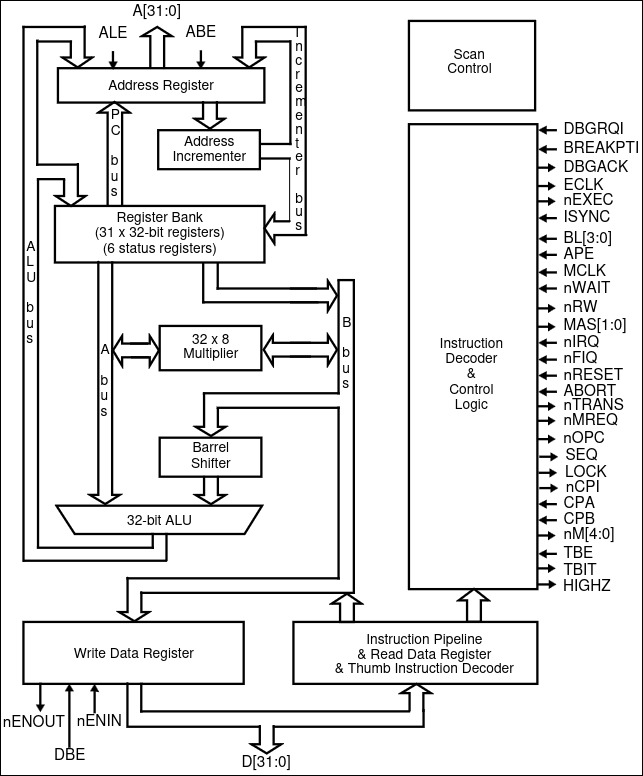
\includegraphics[width=0.6\textwidth]{cpu_diagram.png}
    \caption{Diagrama de blocos interno do núcleo ARM7TDMI, com o
        \textit{datapath} (registrador de endereços, incrementador, banco de
        registradores, multiplicador, \textit{barrel shifter} e ALU de
        32~bits) e a unidade de decodificação e controle, à direita.
        Fonte: ARM Limited~\cite{ARM_DDI0210B}.}
    \label{fig:arm7tdmi}
\end{figure}

\subsection{Arquitetura do Game Boy Advance}

O GBA é, em essência, um sistema-em-chip que combina o ARM7TDMI
operando a 16{,}78~MHz, 96~KiB de VRAM, 32~KiB de IWRAM, 256~KiB
de EWRAM, registradores de I/O memorizados em uma região dedicada
\texttt{0x04000000}, uma PPU com seis modos gráficos, quatro canais
DMA e uma unidade de áudio com canais PSG e canais
PCM~\cite{Copetti2019,Vijn_Tonc,GBATEK}. A interface com o cartucho
(\textit{Game Pak}) ocupa a região \texttt{0x08000000}-\texttt{0x0DFFFFFF}
do mapa de memória, em barramento de 16~bits com modos de acesso
configuráveis em latência~\cite{GBATEK}. Esses parâmetros estabelecem
o conjunto-alvo a ser reproduzido neste trabalho. A
Figura~\ref{fig:gba-arch} resume essa organização interna, destacando os
blocos funcionais e a largura nominal de barramento de cada região.

\begin{figure}[htbp]
    \centering
    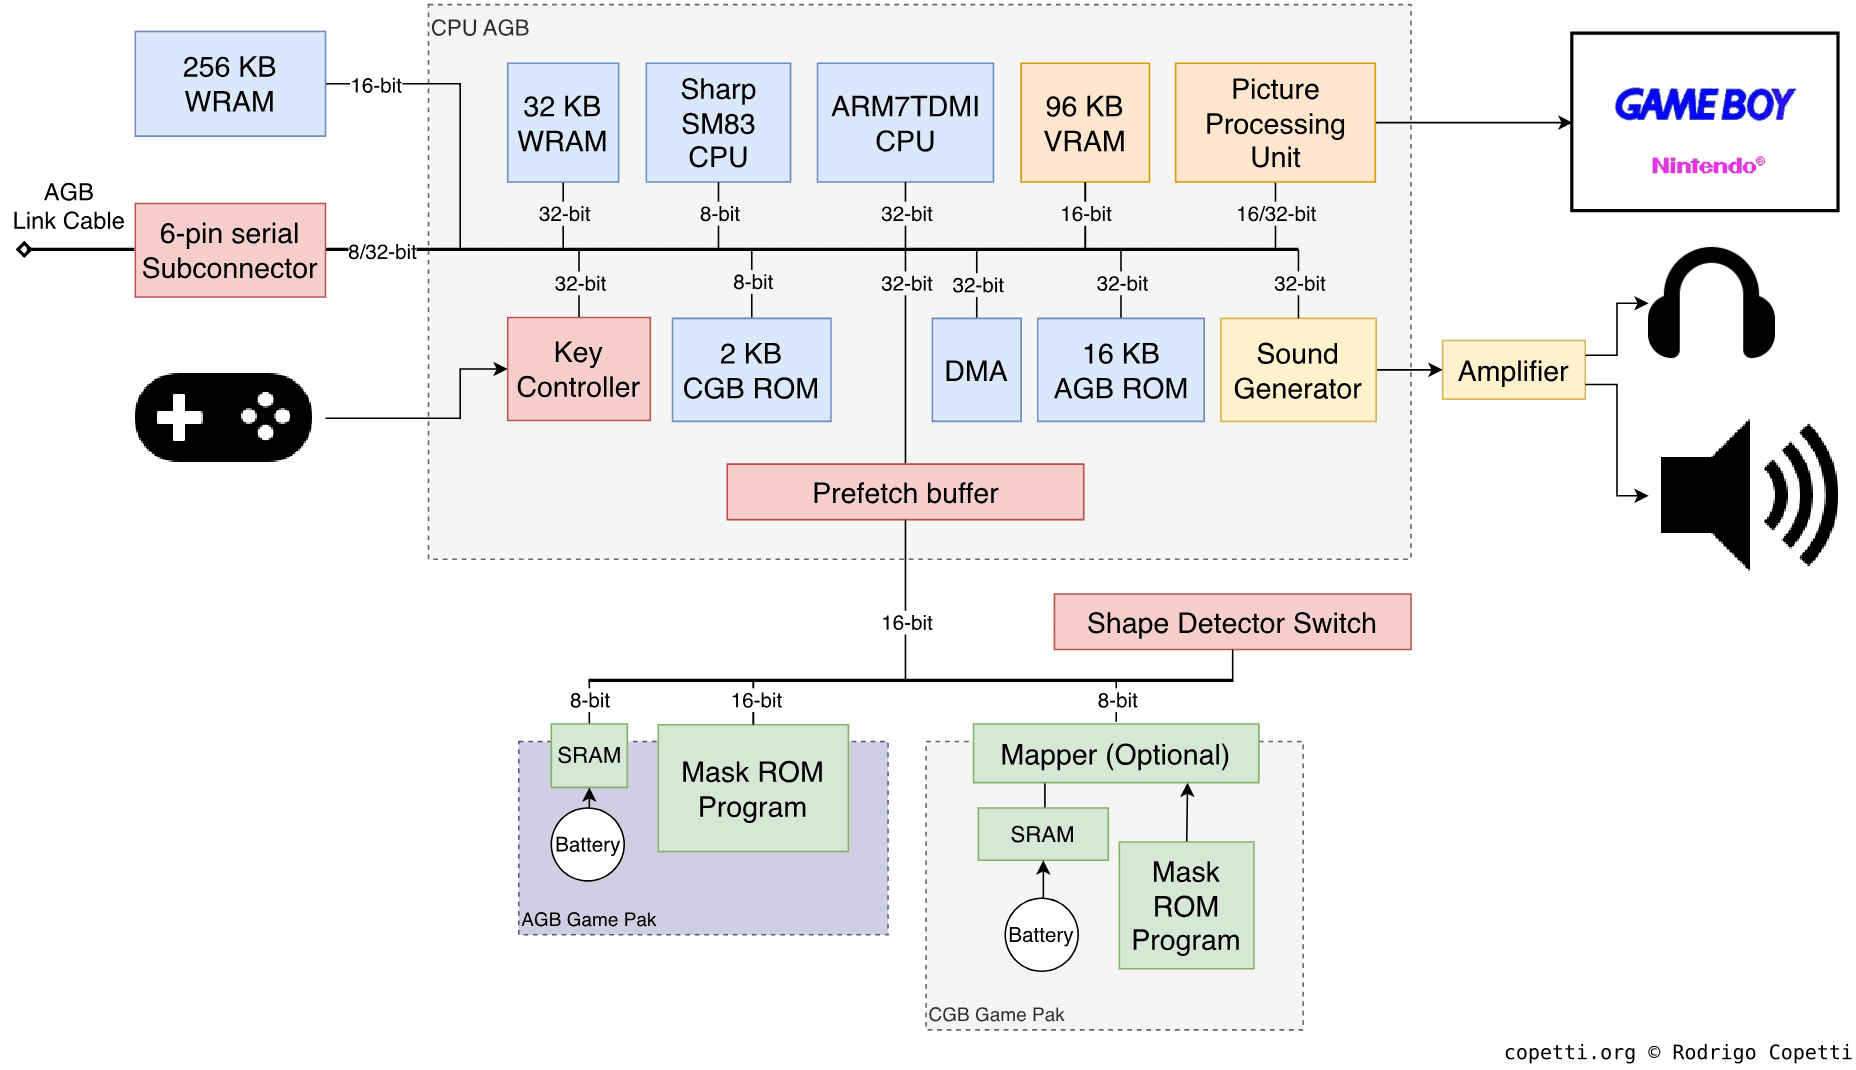
\includegraphics[width=0.95\textwidth]{gba_diagram.png}
    \caption{Arquitetura interna do Game Boy Advance (\textit{die} CPU~AGB):
        núcleo ARM7TDMI, co-processador Sharp~SM83 (retrocompatibilidade), as
        regiões de memória (WRAM interna e externa, VRAM), a PPU, o gerador de
        som, o controlador de DMA e a interface com o \textit{Game Pak};
        indicam-se as larguras de barramento de cada bloco.
        Fonte: Copetti~\cite{Copetti2019}.}
    \label{fig:gba-arch}
\end{figure}


\section{Abordagem Teórica}
\label{sec:abordagem-teorica}

A reprodução de uma arquitetura legada em FPGA admite, em princípio,
três níveis de fidelidade. No nível mais básico, a reprodução
\emph{funcional} (a) executa corretamente o conjunto de instruções e
respeita o mapa de memória, mas mantém a temporização livre; é
apropriada para fins didáticos e como ponto de partida da
verificação. Um passo adiante, a reprodução \emph{ciclo-aproximada}
(b) acrescenta a essa funcionalidade a reprodução da contagem de
ciclos de cada instrução conforme a especificação original. No nível
mais exigente, a reprodução \emph{ciclo-perfeita} (c) reproduz o
comportamento ciclo a ciclo de todos os blocos, incluindo PPU, DMA
e barramento, a ponto de tornar indistinguíveis, do ponto de
vista do software, o original e a reprodução; é o padrão buscado por
projetos como o MiSTer FPGA~\cite{MiSTer}. O presente trabalho almeja
inicialmente a faixa (a)--(b), com uma arquitetura aberta à evolução
incremental rumo a (c) em trabalhos futuros.


\section{Soluções Existentes}
\label{sec:solucoes}

A literatura técnica e a comunidade de \textit{homebrew} oferecem
diversas referências de reprodução do GBA, com diferentes compromissos
de fidelidade e propósito. No campo da emulação em software, o
mGBA~\cite{mGBA}, escrito em C, destaca-se pela altíssima
compatibilidade e pela ampla instrumentação para depuração, enquanto o
NanoBoyAdvance~\cite{NanoBoyAdvance}, em C++, prioriza a precisão
ciclo-aproximada e a legibilidade do código, o que o torna referência
frequente para implementadores em hardware. No campo do hardware
reconfigurável, o núcleo GBA do projeto MiSTer FPGA~\cite{MiSTer}
persegue a alta fidelidade e a execução ciclo-perfeita sobre uma
Cyclone~V do tipo DE10-Nano, ao passo que o Analogue
Pocket~\cite{AnaloguePocket} (Figura~\ref{fig:pocket}), produto comercial
baseado em FPGA, reproduz Game Boy, Game Boy Color e Game Boy Advance e
demonstra a viabilidade industrial da abordagem. Dão suporte a todas essas
iniciativas a documentação de comunidade consolidada na engenharia
reversa do hardware, com destaque para o GBATEK~\cite{GBATEK} e o
Tonc~\cite{Vijn_Tonc}, referência \textit{de facto} para qualquer
reprodução. No domínio acadêmico, projetos de reprodução de CPUs ARM
em FPGA são bem documentados na literatura de ensino de arquitetura de
computadores~\cite{HarrisHarris,PattersonHennessy}, ainda que
normalmente restritos a subconjuntos do ISA; a combinação de um
ARM7TDMI completo com o subsistema gráfico do GBA permanece, contudo,
um nicho explorado majoritariamente pela comunidade de
\textit{retrocomputing}.

\begin{figure}[htbp]
    \centering
    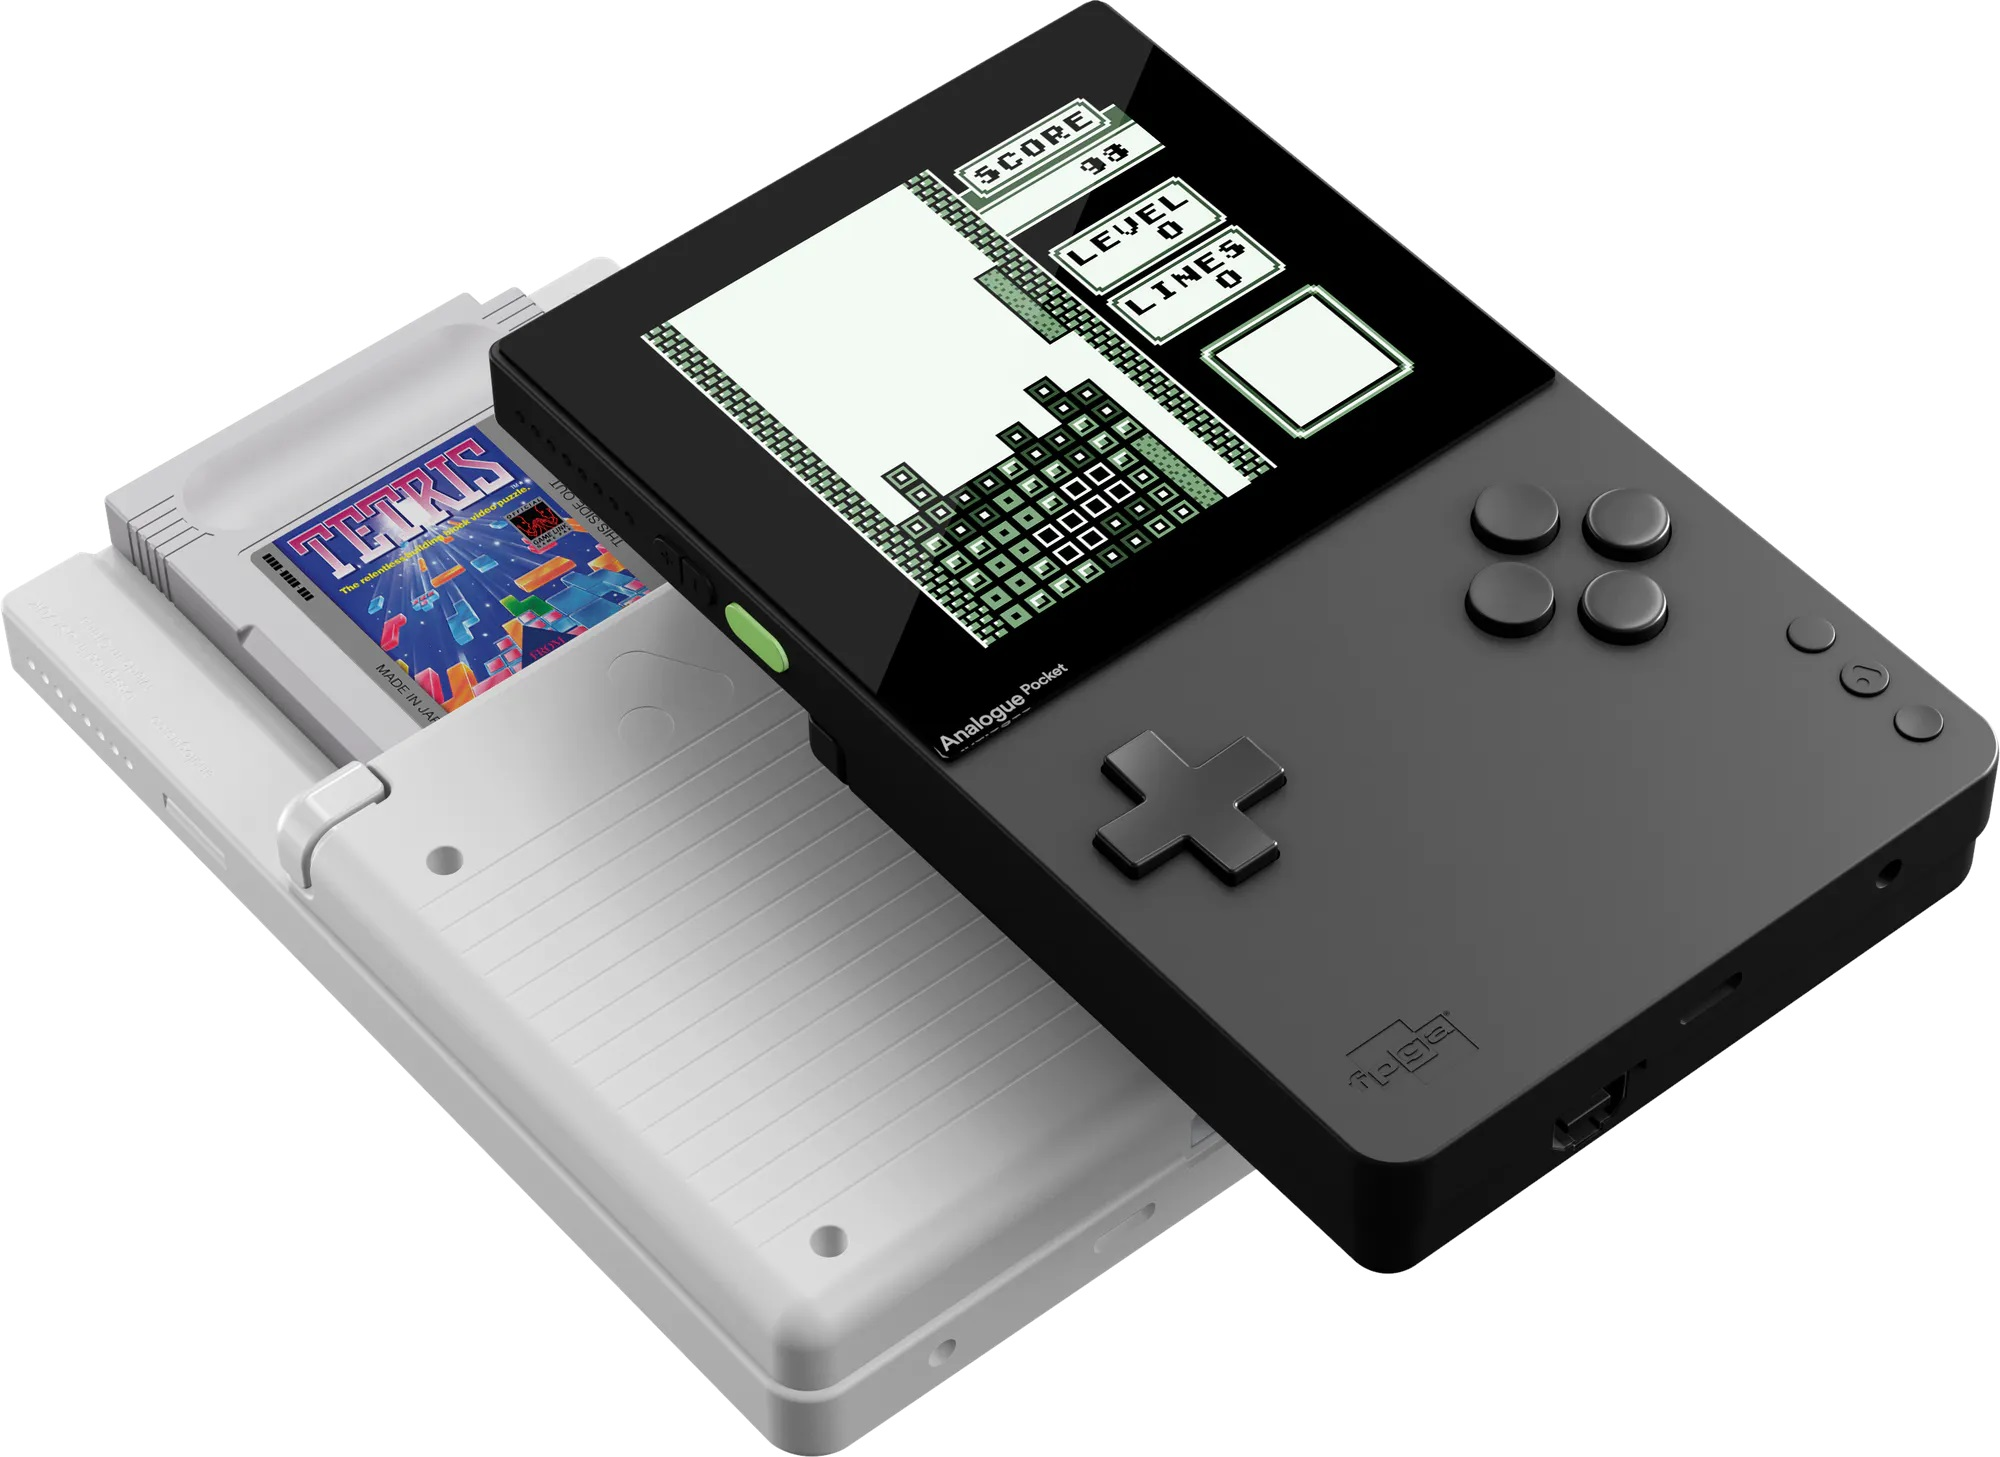
\includegraphics[width=0.6\textwidth]{analogue_pocket.jpg}
    \caption{Analogue Pocket, console portátil comercial baseado em FPGA que
        reproduz Game Boy, Game Boy Color e Game Boy Advance a partir de
        cartuchos originais.
        Fonte: Analogue Inc.~\cite{AnaloguePocket}.}
    \label{fig:pocket}
\end{figure}


\section{Tendências}
\label{sec:tendencias}

Três tendências balizam o estado da arte e o posicionamento deste
trabalho. A primeira é o avanço do \emph{open hardware} e a abertura
de \textit{toolchains}: a crescente disponibilidade de fluxos abertos
para FPGA, como Yosys e nextpnr, para famílias selecionadas, e
de plataformas didáticas a preços decrescentes amplia a base de
pesquisadores capazes de reproduzir arquiteturas~\cite{Trimberger2015}.
A segunda é a consolidação de \textit{cores} reconfiguráveis
colaborativos: projetos como o MiSTer~\cite{MiSTer} demonstram que
reproduções ciclo-perfeitas podem ser construídas de forma incremental
e mantidas por uma comunidade ampla. A terceira é a preservação
digital: agências de preservação cultural reconhecem cada vez mais a
importância de preservar não apenas o software, mas também o
\emph{comportamento} do hardware sobre o qual ele roda, e a reprodução
em FPGA é o veículo técnico mais alinhado a esse
objetivo~\cite{Copetti2019}.


\section{Conclusão do Capítulo}
\label{sec:conclusao-cap2}

O estado da arte mostra que a reprodução do GBA em FPGA é
viável e desejável, com referências técnicas amplas
(documentação ARM~\cite{ARM_DDI0210B,ARM_DVI0027B}, mapa de
memória e periféricos~\cite{GBATEK,Vijn_Tonc,Copetti2019}) e
exemplos práticos consolidados~\cite{MiSTer,AnaloguePocket}.
O espaço para contribuição original deste trabalho situa-se em
duas frentes: a construção pedagógica de uma reprodução completa,
com código aberto, documentado em português e desenvolvido em
plataforma didática consolidada (DE1-SoC); e a demonstração de que
a graduação em Engenharia Elétrica oferece base suficiente para a
execução de um projeto desta natureza.


\chapter{Materiais e Métodos}
\label{cap:materiais-metodos}

Este capítulo descreve a plataforma, as ferramentas e o método de
desenvolvimento e verificação adotados no projeto, bem como a Prova de
Conceito que o materializa. Como a presente monografia acompanha uma
\textbf{entrega intermediária} do Trabalho de Conclusão de Curso, a
descrição da Prova de Conceito reflete o estágio atual do
desenvolvimento: distingue-se, ao longo do texto, aquilo que já foi
implementado e validado, e que constitui a demonstração apresentada
neste momento, daquilo que se encontra em andamento ou planejado
para a entrega final.

\section{Plataforma de Implementação}
\label{sec:plataforma}

A implementação é realizada na placa Altera DE1-SoC, da
Terasic~\cite{TerasicDE1SoC} (Figura~\ref{fig:de1soc}), que abriga uma FPGA
Cyclone~V (\mbox{5CSEMA5F31C6}~\cite{CycloneV}). Entre os recursos da placa
relevantes ao projeto, destacam-se os 64~MiB de SDRAM externa de
16~bits, que abriga a ROM de cartucho (\texttt{PAK\_ROM}) e a EWRAM,
sendo a \texttt{PAK\_ROM} a região que, na fase final do projeto, poderá
ser \emph{escrita} para carregar uma ROM a partir de um cartão SD,
e os blocos M10K de memória \textit{on-chip}, que hospedam as demais
regiões internas do mapa (BIOS, IWRAM, Palette RAM, VRAM e OAM). A saída VGA,
com DAC de 8 bits por canal, serve à interface gráfica, enquanto os
quatro \textit{push-buttons}, os dez \textit{switches}, os LEDs e os
seis \textit{displays} de sete segmentos são empregados na depuração e
na injeção de estímulos, por exemplo, \texttt{KEY[0]} como
\textit{reset}, \texttt{KEY[1..3]} como nIRQ/nFIQ/Abort e
\texttt{SW[9]} como \textit{trigger} do SignalTap. Por fim, a PLL
interna deriva a frequência inicial de operação do núcleo, com divisão
programável que permite reduzi-la a níveis convenientes para a
depuração visual.

\begin{figure}[htbp]
    \centering
    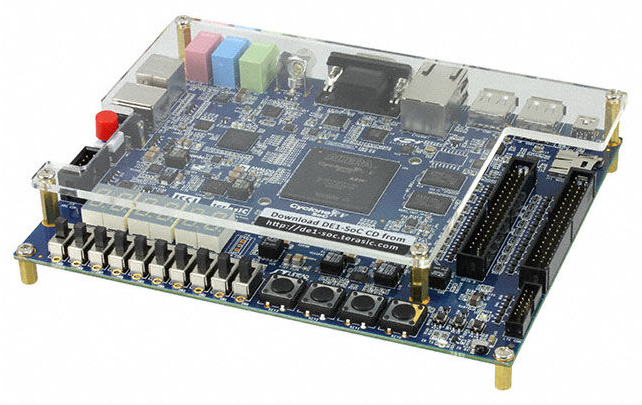
\includegraphics[width=0.7\textwidth]{de1-soc.png}
    \caption{Placa de desenvolvimento Terasic DE1-SoC, baseada na FPGA
        Cyclone~V \mbox{5CSEMA5F31C6}, utilizada como plataforma de
        implementação e depuração do projeto.
        Fonte: Terasic~\cite{TerasicDE1SoC}.}
    \label{fig:de1soc}
\end{figure}


\section{Fluxo de Projeto e Ferramentas}
\label{sec:fluxo}

O fluxo de desenvolvimento articula um conjunto de ferramentas
consolidadas. A síntese, o \textit{place-and-route}, a análise
temporal e a geração do \textit{bitstream} cabem ao Quartus Prime
15.1~\cite{CycloneV}, enquanto a simulação RTL funcional é conduzida no
ModelSim/QuestaSim sobre o topo de simulação \texttt{gba\_rev0\_sim}, um
gêmeo \textit{board-less} do topo de síntese gerado por NativeLink, que
carrega o programa de teste a partir de um arquivo MIF. Os \textit{cores} de PLL, de controle de
\textit{clock} e de SignalTap são gerados no Qsys/Platform Designer. A
geração dos programas de teste, em ARM e Thumb, parte de código
\textit{assembly} processado pela toolchain \texttt{arm-none-eabi}
(\texttt{as}, \texttt{ld} e \texttt{objcopy}) e posteriormente
convertido em formato MIF para a inicialização das memórias
\textit{on-chip}. A verificação em hardware, por sua vez, apoia-se no
SignalTap, com \textit{taps} sobre os registradores $r_0$--$r_{15}$ e
sobre os barramentos de endereços e de dados.


\section{Descrição da Prova de Conceito}
\label{sec:poc}

A Prova de Conceito consiste na execução, na placa DE1-SoC, de
programas binários compilados pela toolchain ARM, com observação
direta do estado do processador via SignalTap e dos \textit{displays}
HEX e, na etapa final do projeto, com exibição em monitor VGA. Para
fins de organização, o sistema é concebido em quatro camadas,
núcleo, memória, vídeo e integração, que avançam de modo
incremental; a Figura~\ref{fig:arquitetura} sintetiza a
\emph{arquitetura-objetivo} do projeto, destacando, por meio de cores,
aquilo que já se encontra implementado e validado, o que está em
desenvolvimento e o que permanece planejado. \textbf{No estágio correspondente a esta entrega
intermediária, a primeira camada já está concluída e validada, e é ela
que constitui a demonstração ora apresentada}; as demais encontram-se
em desenvolvimento ou planejadas, conforme detalhado a seguir.

\subsection{Camada 1: Núcleo ARM7TDMI (implementada e validada)}

A camada mais interna corresponde à descrição RTL do núcleo,
organizada em módulos Verilog independentes, \texttt{arm7tdmi\_top},
\texttt{decoder}, \texttt{reg\_bank}, \texttt{alu},
\texttt{b\_shifter}, \texttt{multiplier}, \texttt{incrementer},
\texttt{address\_reg} e \texttt{write\_data\_reg}. O \texttt{decoder}
concentra a máquina de estados multi-ciclo do processador, controlando
os sinais de habilitação e seleção dos demais blocos e conduzindo o
tratamento de exceções (vetores de Reset, Undefined, SWI, Prefetch
Abort, Data Abort, IRQ e FIQ), ao passo que o \texttt{reg\_bank}
implementa os bancos de registradores espelhados por modo, incluindo o
banco completo de FIQ. Esta camada já se encontra implementada e
validada por meio de programas de teste em ARM (\texttt{instrucoes.s}),
Thumb (\texttt{arm7tdmi\_thumb\_test.s}) e de exceções
(\texttt{interrupt\_test.s}), tanto em simulação no QuestaSim quanto em
execução na placa DE1-SoC. É justamente esse núcleo em funcionamento
--- capaz de buscar, decodificar e executar instruções ARM e Thumb e
de responder a interrupções e exceções, com o estado interno
observável via SignalTap e na saída HEX, que materializa a Prova de
Conceito apresentada nesta entrega intermediária. A
Figura~\ref{fig:rtl-atual} apresenta a \textit{netlist} RTL do projeto
no estágio atual, gerada pela ferramenta de síntese, na qual já
coexistem o núcleo ARM7TDMI validado e os blocos do subsistema de
memória em integração.
% [INDICAR: tabelar, na entrega final, quais instruções ARM/Thumb já
%  foram cobertas pelos vetores de teste e quais ainda permanecem em
%  aberto.]

\begin{figure}[htbp]
    \centering
    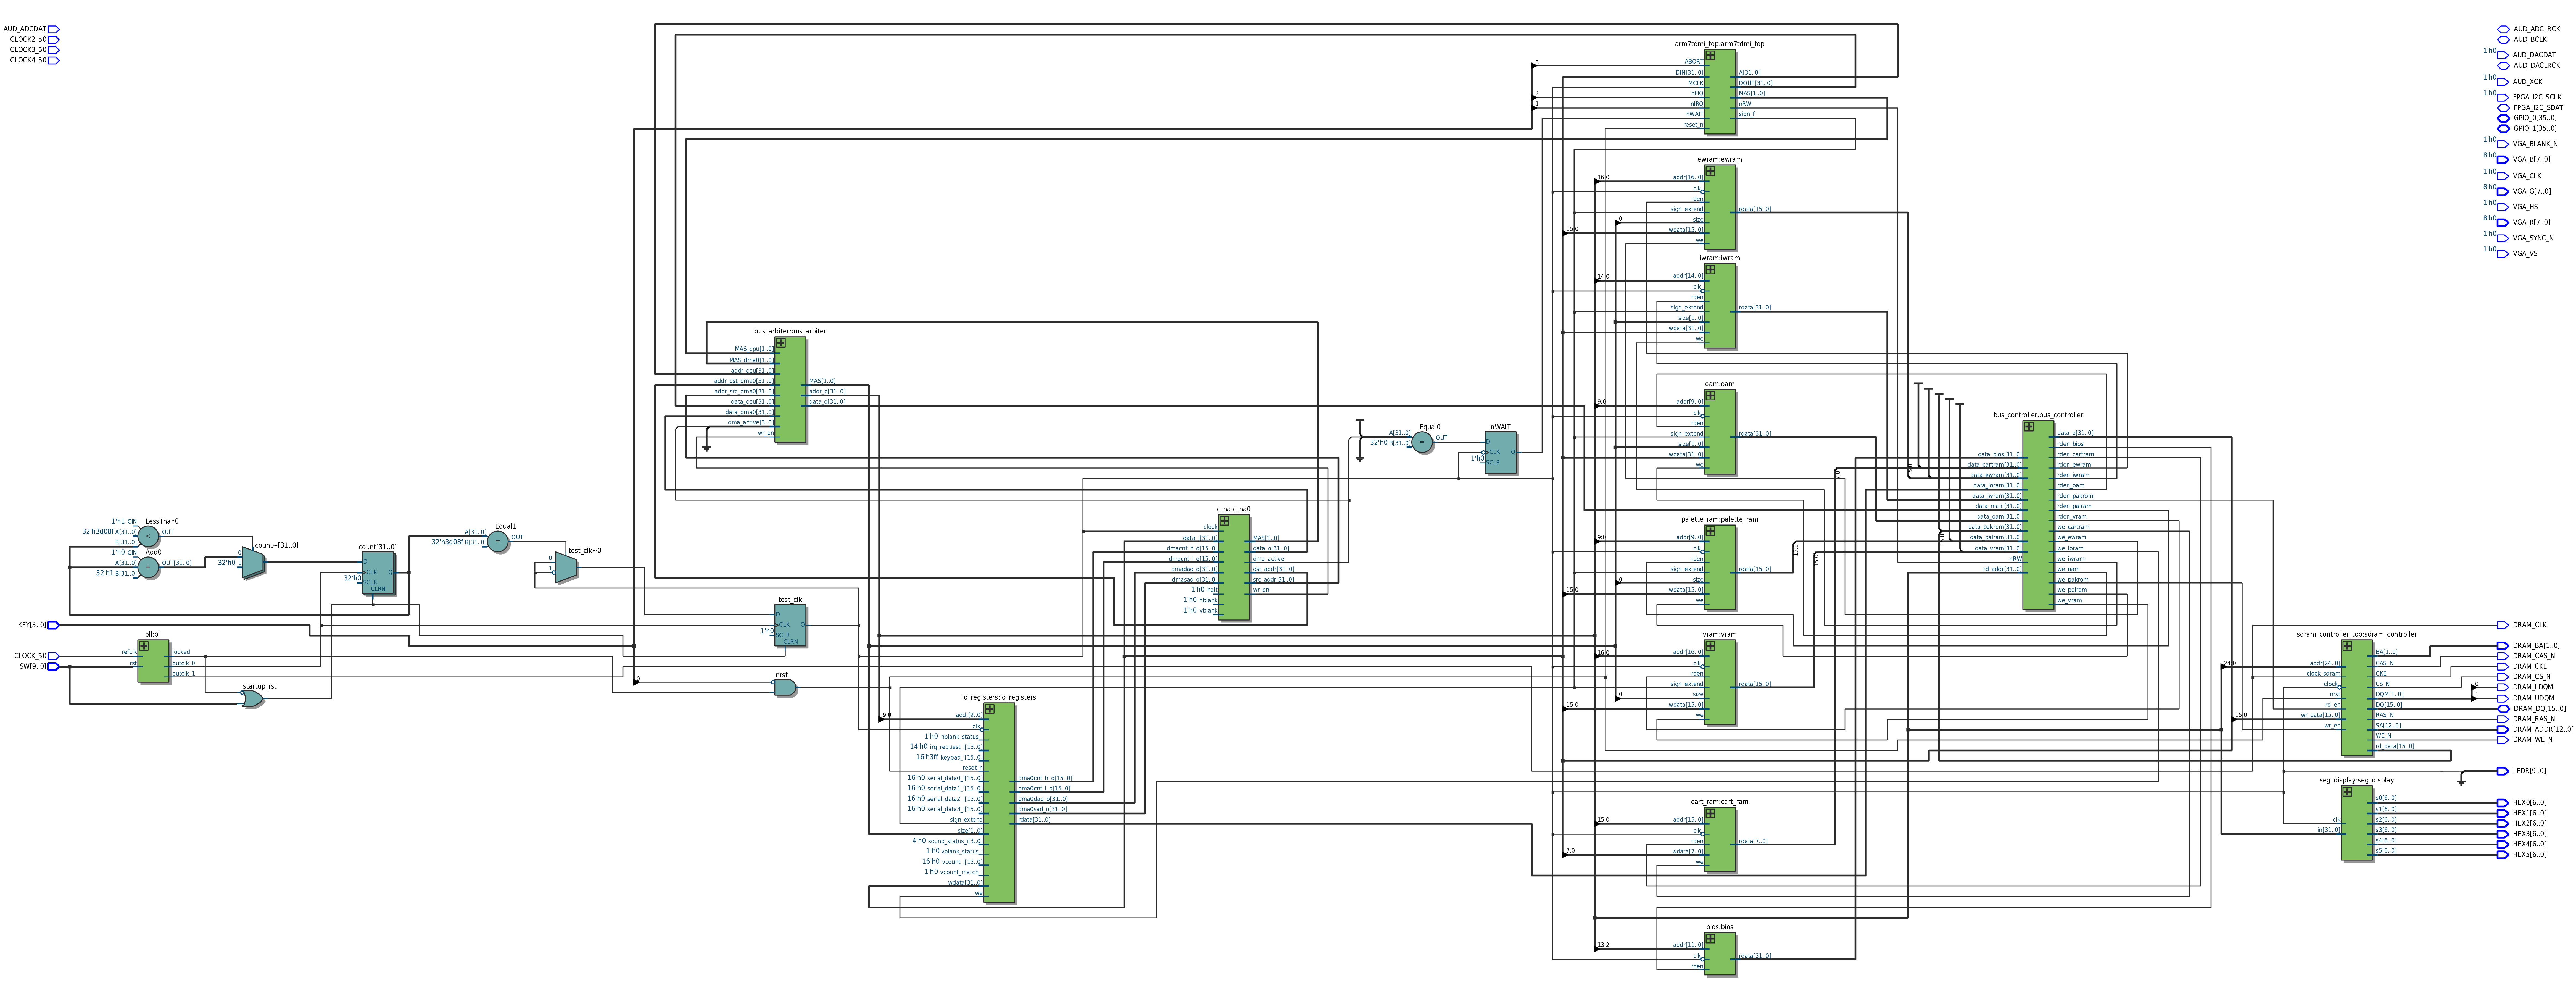
\includegraphics[width=\textwidth]{rtl_atual.png}
    \caption{\textit{Netlist} RTL do projeto no estágio atual, extraída pelo
        \textit{RTL Viewer} do Quartus Prime após a análise e síntese. Reúne o
        núcleo ARM7TDMI já implementado e validado e os blocos do subsistema de
        memória ainda em integração (\texttt{bus\_controller}, módulos de
        região e controlador de SDRAM). Fonte: autoria própria.}
    \label{fig:rtl-atual}
\end{figure}

\subsection{Camada 2: Subsistema de Memória (integrada, em validação)}

A camada de memória encontra-se descrita e \emph{integrada} ao
\textit{datapath} do sistema, embora a validação funcional do caminho
integrado ainda esteja em andamento. Nesta entrega, o mapa de memória
do GBA, e não mais a SRAM plana provisória que serviu à validação
da Camada~1, constitui o caminho de memória ativo no projeto. O
módulo \texttt{sram.v}, que descreve uma SRAM de 4~KiB inferida em
blocos M10K (com suporte a \textit{byte enables}, alinhamento e
extensão de sinal) e serviu de memória unificada durante a validação
do núcleo, permanece no repositório apenas como referência, desativado
no topo em favor do mapa completo.

A decodificação do mapa cabe ao \texttt{bus\_controller.v}, que
interpreta o \textit{nibble} alto do endereço (\texttt{addr[27:24]}),
gera os sinais de \emph{read}/\emph{write enable} por região e
multiplexa os dados lidos de volta ao processador. Acima dele, o
\texttt{bus\_arbiter.v} arbitra o acesso ao barramento único entre o
processador e os quatro canais de DMA, ao passo que o módulo
\texttt{dma.v}, instanciado nos quatro canais (DMA0--DMA3), executa as
transferências em bloco a partir dos registradores de controle providos pelo
\texttt{io\_registers.v}. Os módulos de região (\texttt{bios.v},
\texttt{iwram.v}, \texttt{io\_registers.v},
\texttt{palette\_ram.v}, \texttt{vram.v}, \texttt{oam.v} e
\texttt{cart\_ram.v}), inferidos em blocos M10K \textit{on-chip},
modelam cada faixa interna do mapa, com tratamento de tamanho de
acesso e extensão de sinal por região.

A ROM de cartucho (\texttt{PAK\_ROM}) e a EWRAM são as regiões mapeadas na
SDRAM externa da DE1-SoC, servidas por um controlador de SDRAM próprio
(\texttt{sdram\_controller.v} e seu envoltório
\texttt{sdram\_controller\_top.v}), já instanciado no topo do projeto.
Esse controlador, desenvolvido para substituir a IP de referência
antes utilizada, opera o núcleo de acesso à SDRAM em um domínio de
\textit{clock} próprio e realiza a sincronização entre esse domínio e
o domínio do processador por meio de uma lógica de \textit{clock-domain
crossing} com retenção de requisição, de modo que uma transação que
coincida com um ciclo de \textit{refresh} não seja perdida. Sobre o
barramento físico de 16~bits da SDRAM, o controlador suporta acessos de
\textit{byte}, \textit{halfword} e \textit{word} --- estes últimos
realizados como duas meias-transferências sequenciais de 16~bits ---,
com máscara de \textit{bytes} na escrita e extensão de sinal na leitura.
Como a região de \texttt{PAK\_ROM} é escrevível, prevê-se, na fase final
do projeto, utilizá-la para carregar uma ROM a partir de um cartão SD
para a SDRAM.
% [INDICAR: incluir, no Capítulo 3 final, o diagrama de tempo do
%  protocolo SDRAM utilizado, com base no datasheet do dispositivo
%  IS42S16320D montado na DE1-SoC.]

\subsection{Camada 3: Saída de Vídeo (planejada)}

A camada de vídeo, ainda não implementada no momento desta entrega,
compreenderá um gerador VGA com sincronismos horizontal e vertical
para uma resolução padrão (a definir entre 640$\times$480 e
800$\times$600, ambas a 60~Hz), o mapeamento do \textit{framebuffer}
do GBA (240$\times$160) sobre a região visível do monitor com escala
inteira e o suporte inicial ao Modo~3 do console (\textit{bitmap}
16~bpp), o mais simples de implementar e suficiente para demonstrar a
saída de vídeo.
% [INDICAR: discutir, após análise dos recursos disponíveis na
%  Cyclone~V, se a VRAM ficará em M10K ou em SDRAM, e justificar.]

\subsection{Camada 4: Integração e Validação (planejada)}

A camada de integração reunirá as três anteriores em uma arquitetura
única, instanciando o \texttt{arm7tdmi\_top} sobre o
\texttt{bus\_controller} e este sobre as memórias e periféricos. Sua
validação se dará pela execução de programas de teste em
\textit{assembly} cobrindo categorias específicas de instruções,
estratégia já adotada na Camada~1, pela execução de uma ROM
\textit{homebrew} de baixo porte como demonstração final, com saída de
vídeo no monitor VGA, e pela comparação cruzada do comportamento
observado em FPGA com o do emulador NanoBoyAdvance~\cite{NanoBoyAdvance}
executando a mesma ROM, tomado como referência funcional.


\section{Metodologia de Verificação}
\label{sec:verificacao}

A verificação apoia-se em três níveis complementares. O primeiro é a
simulação RTL no QuestaSim, conduzida sobre o topo de simulação
\texttt{gba\_rev0\_sim} --- um gêmeo \textit{board-less} do topo de
síntese, clocado diretamente e carregado com o programa de teste ---,
com inspeção das formas de onda dos barramentos, dos registradores do
\texttt{reg\_bank}, do \textit{datapath} interno do \texttt{decoder} e
dos sinais de controle. O segundo é a execução em hardware na DE1-SoC,
com captura, via SignalTap, dos registradores $r_0$--$r_{15}$ e dos
barramentos de endereços e de dados. O terceiro é a comparação com uma
referência externa: para cada cenário, a sequência de estados esperada
é obtida executando-se o mesmo binário em um emulador de
referência~\cite{mGBA,NanoBoyAdvance}, que assim cumpre o papel de
\textit{golden model}. Cabe observar que, nesta entrega intermediária,
os dois primeiros níveis já se encontram em uso efetivo sobre o núcleo
ARM7TDMI, ao passo que a comparação sistemática contra o
\textit{golden model} será consolidada à medida que as camadas de
memória e vídeo forem integradas.


\section{Cronograma Macro}
\label{sec:cronograma}

O Quadro~\ref{tab:cronograma} apresenta o cronograma macro de execução
do projeto. A presente entrega intermediária corresponde à conclusão
das fases F1 e F2, estudo da arquitetura e implementação RTL do
núcleo ARM7TDMI, com sua validação em simulação e em hardware, e ao
andamento da fase F3, na qual o subsistema de memória já foi descrito
e integrado ao \textit{datapath}, restando a validação funcional do
caminho integrado. O projeto encontra-se, neste momento, na fase F3;
as fases F4 a F6 descrevem, portanto, a continuidade prevista até a
entrega final. O cronograma detalhado, com desdobramento semanal e
marcos intermediários, constitui entrega complementar e está
localizado em
\texttt{documentos\_de\_entrega/Cronograma/cronograma\_detalhado.xlsx},
acompanhado das versões editáveis em \texttt{.csv} e \texttt{.md} na
mesma pasta.

\begin{table}[h]
    \centering
    \caption{Cronograma macro de execução.}
    \label{tab:cronograma}
    \begin{tabular}{@{}clp{0.55\textwidth}@{}}
        \toprule
        \textbf{Fase} & \textbf{Mês} & \textbf{Atividades} \\
        \midrule
        F1 & 1 e 2 &
            Estudo da arquitetura ARM7TDMI e  do mapa de
            memória do GBA. \emph{(concluída)} \\
        F2 & 3 e 4 &
            Implementação RTL do núcleo ARM7TDMI;
            Síntese física do núcleo na DE1-SoC; programas
            de teste em ARM e Thumb; validação por
            SignalTap; tratamento completo de exceções e IRQ/FIQ.
            \emph{(concluída, entrega intermediária)} \\
        F3 & 5 e 6 &
            Subsistema de memória: \texttt{bus\_controller},
            \texttt{bus\_arbiter}, DMA, módulos de região,
            controlador de SDRAM; integração ao núcleo concluída,
            validação funcional do caminho integrado em andamento.
            \emph{(em andamento)} \\
        F4 & 7 e 8 &
            Implementação do PPU e produzir imagem em um display.
            \emph{(previsto)} \\
        F5 & 9 e 10 &
            Implementação do comando do usuário e gerador de som.
            \emph{(previsto)} \\
        F6 & 11 e 12 &
            Validação com um jogo real: transferência de uma ROM de 
            um SD Card para SDRAM. \emph{(previsto)} \\
        % [INDICAR: alinhar os bimestres com o calendário
        %  acadêmico oficial e ajustar caso o projeto se
        %  estenda além de 2027.]
        \bottomrule
    \end{tabular}
\end{table}

\begin{figure}[htbp]
    \centering
    \resizebox{\textwidth}{!}{%
    \begin{tikzpicture}[
        font=\small,
        >={Stealth[length=2.2mm]},
        core/.style ={draw, thick, rounded corners, fill=blue!12,
                      minimum width=28mm, minimum height=13mm, align=center},
        mem/.style  ={draw, thick, rounded corners, fill=orange!14,
                      minimum width=17mm, minimum height=12mm, align=center,
                      font=\scriptsize},
        ext/.style  ={draw, thick, rounded corners, fill=orange!14,
                      minimum width=23mm, minimum height=12mm, align=center,
                      font=\scriptsize},
        plan/.style ={draw, thick, dashed, rounded corners, fill=gray!12,
                      minimum width=16mm, minimum height=11mm, align=center,
                      font=\scriptsize, text=black},
        wlbl/.style ={midway, fill=white, inner sep=1.15pt, font=\scriptsize},
        bus2/.style ={<->, thick},
        rd/.style   ={->, thick},
    ]
    \coordinate (O) at (0,0);

    % ===================== System bus =====================
    \draw[line width=1.4mm, gray!55] (-1.2,0) -- (18.6,0);
    \node[anchor=north west, font=\scriptsize\itshape] at (-1.2,-0.25)
        {Barramento de sistema (32\,bits)};

    % ===================== Masters (above the bus) =====================
    \node[core] (cpu) at (6.0,3.2) {\textbf{ARM7TDMI}\\\scriptsize núcleo (\texttt{arm7tdmi\_top})};
    \node[mem] (arb) at (9.0,3.2) {\textbf{Bus}\\\textbf{Arbiter}};
    \node[mem] (dma) at (11.5,3.2) {\textbf{DMA}};
    \node[mem]  (bcl) at (9.0,1.25) {\textbf{Bus}\\\textbf{Controller}};

    \draw[bus2] (cpu.east) -- (arb.west);
    \draw[bus2] (dma.west) -- (arb.east);
    \draw[->, thick] (arb.south) -- (bcl.north);

    % PPU container (planned) wrapping PAL + OAM (in development)
    \node[plan, minimum width=46mm, minimum height=20mm] (ppu) at (15.4,3.35) {};
    \node[anchor=north, font=\scriptsize\bfseries] at ([yshift=-0.5mm]ppu.north) {PPU};
    \node[mem, minimum width=15mm, minimum height=10mm] (pal) at (14.3,2.95)
        {\textbf{Palette}\\1\,KiB\\16\,bits};
    \node[mem, minimum width=15mm, minimum height=10mm] (oam) at (16.5,2.95)
        {\textbf{OAM}\\1\,KiB\\32\,bits};

    \node[plan, minimum width=17mm] (disp) at (20.6,3.35) {\textbf{Display}\\(VGA ou LCD)};
    \draw[rd] (ppu.east) -- (disp.west);

    \node[plan, minimum width=22mm] (snd) at (15.9,-2.8) {\textbf{Sound Generator}};
    \node[plan, minimum width=16mm] (aud) at (20.6,-2.8) {\textbf{Áudio}};
    \draw[rd] (snd.east) -- (aud.west);

    %, master taps onto the bus,
    \draw[bus2] (cpu.south) -- (cpu  |- O) node[wlbl,right]{32\,b};
    \draw[bus2] (dma.south) -- (dma  |- O) node[wlbl,right]{32\,b};
    \draw[->, thick] (bcl.south) -- (bcl |- O);
    \draw[bus2] (ppu.south) -- (ppu  |- O) node[wlbl,right]{16/32\,b};
    \draw[bus2] (snd.north) -- (snd  |- O) node[wlbl,right]{32\,b};

    % ===================== Cartridge / external (top-left) =====================
    \node[ext] (pakrom) at (3.1,4.7) {\textbf{SDRAM}\\PAK\_ROM\\(externa)};
    \node[ext] (ewram) at (-0.2,2.75) {\textbf{SDRAM}\\EWRAM\\(externa)};
    \node[ext] (sdramc) at (3.1,2.75) {\textbf{SDRAM}\\\textbf{Controller}};

    \node[mem, minimum width=15mm] (pakram) at (-0.1,1.25) {\textbf{PAK\_RAM}\\(save)};

    \draw[bus2] (pakrom.south) -- (sdramc.north) node[wlbl,right]{16\,b};
    \draw[bus2] (ewram.east)   -- (sdramc.west) node[wlbl,above]{16\,b};
    \draw[bus2] (pakram.south) -- (pakram |- O) node[wlbl,right]{8\,b};
    \draw[bus2] (sdramc.south) -- (sdramc |- O);

    % ===================== Slaves (below the bus) =====================
    \node[plan, minimum width=15mm] (userin)  at (1.8,-2.8) {\textbf{User}\\\textbf{Input}};
    \node[plan, minimum width=15mm] (keyctrl) at (4.4,-2.8) {\textbf{Key}\\\textbf{Controller}};
    \node[mem] (bios)  at (6.8,-2.8)  {\textbf{BIOS}\\16\,KiB};
    \node[mem] (iwram) at (9.0,-2.8)  {\textbf{IWRAM}\\32\,KiB};
    \node[mem] (vram)  at (11.2,-2.8) {\textbf{VRAM}\\96\,KiB};
    \node[mem, minimum width=18mm] (io) at (13.4,-2.8) {\textbf{I/O}\\registradores};
    %\node[mem, minimum width=18mm] (io) at (15.9,-2.8) {\textbf{I/O}\\registradores};

    \draw[rd] (userin.east) -- (keyctrl.west);
    \draw[bus2] (keyctrl.north) -- (keyctrl |- O);
    \foreach \n / \x in {bios/32,iwram/32,vram/16,io/16}{
        \draw[bus2] (\n.north) -- (\n |- O) node[wlbl,right]{\x\,b};
    }

    % ===================== Legend =====================
    \node[draw, thick, fill=blue!12, minimum width=6mm, minimum height=3.5mm,
          anchor=north west] (l1) at (-1.2,-4.4) {};
    \node[anchor=west, font=\scriptsize, right=1.5mm of l1]
        {\textbf{Implementado e validado:} núcleo ARM7TDMI (Camada~1)};
    \node[draw, thick, fill=orange!14, minimum width=6mm, minimum height=3.5mm,
          below=2.5mm of l1] (l2) {};
    \node[anchor=west, font=\scriptsize, right=1.5mm of l2]
        {\textbf{Implementado e integrado:} subsistema de memória (\texttt{bus\_controller}, regiões internas, \texttt{PAK\_RAM} e controlador de SDRAM), arbitragem de barramento e DMA};
    \node[draw, thick, dashed, fill=gray!12, minimum width=6mm, minimum height=3.5mm,
          below=2.5mm of l2] (l3) {};
    \node[anchor=west, font=\scriptsize, right=1.5mm of l3]
        {\textbf{Planejado:} PPU/saída de vídeo, gerador de som/áudio e interface de entrada};
    \end{tikzpicture}%
    }
    \caption{Arquitetura-objetivo do projeto. O núcleo ARM7TDMI (azul) já se encontra implementado e
        validado; o subsistema de memória (laranja), \texttt{bus\_controller},
        regiões internas (BIOS, IWRAM, VRAM, I/O, Palette, OAM),
        \texttt{PAK\_RAM} e o controlador da SDRAM externa, que abriga
        a \texttt{PAK\_ROM} e a EWRAM, além da arbitragem de barramento e dos quatro canais de DMA,
        encontra-se implementado e integrado ao \textit{datapath}, com a validação funcional
        do caminho integrado ainda em andamento; os blocos
        de PPU e saída de vídeo, gerador de som e áudio, e a interface de entrada (\textit{Key Controller}) permanecem
        planejados (cinza). As larguras indicadas correspondem ao barramento
        nominal de cada região; a decodificação por região emprega o
        \textit{nibble} alto do endereço (\texttt{addr[27:24]}).}
    \label{fig:arquitetura}
\end{figure}

% [INDICAR: incluir, na versão final, um diagrama de tempo simplificado
%  mostrando o ciclo Fetch--Decode--Execute do ARM7TDMI no projeto, em
%  complemento ao diagrama de blocos da Figura~\ref{fig:arquitetura}.]


% ========== Referências (ABNT NBR 6023, via abntex2cite) ==========
% Entradas mantidas em referencias.bib; estilo numérico (abntex2-num)
% é carregado pela opção [num] de abntex2cite no preâmbulo.
\bibliography{referencias}


% ========== Apêndices (opcional) ==========
% [INDICAR: incluir como apêndice, na versão final,
%  o \textit{listing} reduzido dos módulos
%  \texttt{arm7tdmi\_top.v}, \texttt{decoder.v} e
%  \texttt{reg\_bank.v}, bem como o \texttt{.qsf}
%  resumido, para fins de reprodutibilidade.]
%\apendice
%\chapter{Listagens de código}

% ========== Anexos (opcional) ==========
% [INDICAR: anexar os relatórios do Quartus
%  (\texttt{gba\_rev0.fit.summary} e
%  \texttt{gba\_rev0.sta.summary}) após o
%  fechamento da etapa de síntese final.]
%\anexo
%\chapter{Relatórios de síntese e timing}


\end{document}
